This test case repeats the exercise from Case~1a using a vulnerability model with nonzero coefficients of variation. Table~\ref{tab:vf-ln-tax1-nzcov} shows the mean loss ratios and corresponding coefficients of variation for the vulnerability function used in this test case.

Apart from the computation of the conditional loss ratio exceedance matrix, the steps for computing the loss exceedance curve in this case are the same as those employed in Case~1a. The conditional loss ratio exceedance matrix in this case is populated by evaluating the complementary cumulative distribution function (CCDF) of the lognormal distribution at each of the prescribed intensity levels, for the set of loss ratios.

\begin{table}[htbp]

\centering
\begin{tabular}{ l c c c c c c c c c }

\hline
\rowcolor{anti-flashwhite}
\bf{LR | PGA} & \bf{0.05g} & \bf{0.20g} & \bf{0.40g} & \bf{0.60g} & \bf{0.80g} & \bf{1.00g} & \bf{1.20g} & \bf{\dots} & \bf{2.00g} \\
\hline
\bf{0.01} & 0.494 & 1.000 & 1.000 & 1.000 & 1.000 & 1.000 & 1.000 & \dots & 1.000 \\
\bf{0.04} & 0.000 & 0.476 & 1.000 & 1.000 & 1.000 & 1.000 & 1.000 & \dots & 1.000 \\
\bf{0.10} & 0.000 & 0.000 & 0.453 & 0.980 & 0.999 & 1.000 & 1.000 & \dots & 1.000 \\
\bf{0.20} & 0.000 & 0.000 & 0.001 & 0.438 & 0.881 & 0.986 & 0.999 & \dots & 1.000 \\
\bf{0.33} & 0.000 & 0.000 & 0.000 & 0.039 & 0.427 & 0.812 & 0.959 & \dots & 1.000 \\
\bf{0.50} & 0.000 & 0.000 & 0.000 & 0.001 & 0.094 & 0.424 & 0.730 & \dots & 1.000 \\
\bf{0.67} & 0.000 & 0.000 & 0.000 & 0.000 & 0.017 & 0.170 & 0.427 & \dots & 1.000 \\
\bf{0.80} & 0.000 & 0.000 & 0.000 & 0.000 & 0.005 & 0.079 & 0.253 & \dots & 1.000 \\
\bf{0.90} & 0.000 & 0.000 & 0.000 & 0.000 & 0.002 & 0.043 & 0.162 & \dots & 0.999 \\
\bf{0.96} & 0.000 & 0.000 & 0.000 & 0.000 & 0.001 & 0.030 & 0.122 & \dots & 0.844 \\
\bf{0.99} & 0.000 & 0.000 & 0.000 & 0.000 & 0.001 & 0.025 & 0.106 & \dots & 0.494 \\
\bf{1.00} & 0.000 & 0.000 & 0.000 & 0.000 & 0.001 & 0.023 & 0.101 & \dots & 0.363 \\
\hline
\end{tabular}

\caption{Conditional loss ratio exceedance matrix for classical risk test case 1c}
\label{tab:lrem-ln-tax1-nzcov}
\end{table}

The loss ratio exceedance matrix in this case is shown in Table~\ref{tab:lrem-ln-tax1-nzcov}.

The loss curve thus calculated above is compared with the loss curve obtained using the OpenQuake classical PSHA based risk calculator in Figure~\ref{fig:lc-cr-1c}.

\begin{figure}[htbp]
\centering
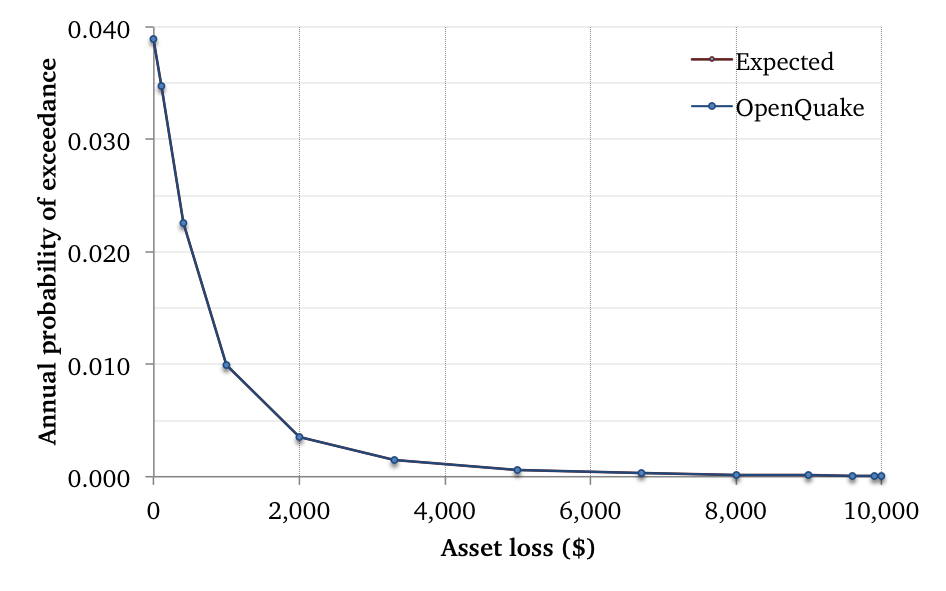
\includegraphics[width=12cm]{qareport/figures/fig-lc-cr-1c}
\caption{Loss curve comparison for classical risk test case 1c}
\label{fig:lc-cr-1c}
\end{figure}

The area under the annual loss exceedance curve gives the average annual loss.